\documentclass[a4paper,14pt]{extreport}
\usepackage[left=1.5cm,right=1.5cm,
    top=1.5cm,bottom=2cm,bindingoffset=0cm]{geometry}
\usepackage{scrextend}
\usepackage[T1,T2A]{fontenc}
\usepackage[utf8]{inputenc}
\usepackage[english,russian,ukrainian]{babel}
\linespread{1.5}
\usepackage{tabularx}
\usepackage{amssymb}
\usepackage{color}
\usepackage{amsmath}
\usepackage{mathrsfs}
\usepackage{listings}
\usepackage{graphicx}
\graphicspath{ {./images/} }
\usepackage{lipsum}
\usepackage{xcolor}
\usepackage{hyperref}
\usepackage{tcolorbox}
\usepackage{tikz}
\usepackage[framemethod=TikZ]{mdframed}
\usepackage{wrapfig,boxedminipage,lipsum}
\mdfdefinestyle{MyFrame}{%
linecolor=blue,outerlinewidth=2pt,roundcorner=20pt,innertopmargin=\baselineskip,innerbottommargin=\baselineskip,innerrightmargin=20pt,innerleftmargin=20pt,backgroundcolor=gray!50!white}
 \usepackage{csvsimple}
 \usepackage{supertabular}
\usepackage{pdflscape}
\usepackage{fancyvrb}
%\usepackage{comment}
\usepackage{array,tabularx}
\usepackage{colortbl}
\usepackage{fp}

\usepackage{varwidth}
\tcbuselibrary{skins}
\usepackage{fancybox}


\usepackage{tikz}
\usepackage[framemethod=TikZ]{mdframed}
\usepackage{xcolor}
\usetikzlibrary{calc}
\makeatletter
\newlength{\mylength}
\xdef\CircleFactor{1.1}
\setlength\mylength{\dimexpr\f@size pt}
\newsavebox{\mybox}
\newcommand*\circled[2][draw=blue]{\savebox\mybox{\vbox{\vphantom{WL1/}#1}}\setlength\mylength{\dimexpr\CircleFactor\dimexpr\ht\mybox+\dp\mybox\relax\relax}\tikzset{mystyle/.style={circle,#1,minimum height={\mylength}}}
\tikz[baseline=(char.base)]
\node[mystyle] (char) {#2};}
\makeatother

\definecolor{ggreen}{rgb}{0.4,1,0}
\definecolor{rred}{rgb}{1,0.1,0.1}
\definecolor{amber}{rgb}{1.0, 0.75, 0.0}
\definecolor{babyblue}{rgb}{0.54, 0.81, 0.94}
\definecolor{amethyst}{rgb}{0.6, 0.4, 0.8}

\usepackage{float}
\usepackage{wrapfig}
\usepackage{framed}
%for nice Code{
\lstdefinestyle{customc}{
  belowcaptionskip=1\baselineskip,
  breaklines=true,
  frame=L,
  xleftmargin=\parindent,
  language=C,
  showstringspaces=false,
  basicstyle=\small\ttfamily,
  keywordstyle=\bfseries\color{green!40!black},
  commentstyle=\itshape\color{purple!40!black},
  identifierstyle=\color{blue},
  stringstyle=\color{orange},
}
\lstset{escapechar=@,style=customc}
%}


\begin{document}
\pagecolor{white}

%----------------------------------------1
\newtcbox{\xmybox}[1][red]{on line, arc=7pt,colback=#1!10!white,colframe=#1!50!black, before upper={\rule[-3pt]{0pt}{10pt}},boxrule=1pt, boxsep=0pt,left=6pt,right=6pt,top=2pt,bottom=2pt}



\begin{titlepage}
  \begin{center}
    \large
    Національний технічний університет України \\ "Київський політехнічний інститут імені Ігоря Сікорського"


    Факультет Електроніки

    Кафедра мікроелектроніки
    \vfill

    \textsc{ЗВІТ}\\

    {\Large Про виконання курсової роботи \\
      з дисципліни: «Твердотільна електроніка-2»\\[1cm]

        Варіант №22


    }
  \bigskip
\end{center}
\vfill

\newlength{\ML}
\settowidth{\ML}{«\underline{\hspace{0.4cm}}» \underline{\hspace{2cm}}}
\hfill
\begin{minipage}{1\textwidth}
Виконавець:\\
Студент 3-го курсу \hspace{4cm} $\underset{\text{(підпис)}}{\underline{\hspace{0.2\textwidth}}}$  \hspace{1cm}Б.\,В.~Лищенко\\
\vspace{1cm}

Превірив: \hspace{6.1cm} $\underset{\text{(підпис)}}{\underline{\hspace{0.2\textwidth}}}$  \hspace{1cm}Л.\,М.~Королевич\\

\end{minipage}

\vfill

\begin{center}
2021
\end{center}
\end{titlepage}
%---------------------------------------------------------------------------------------------------------------------------------------------------------------------------------





\begin{center}Завдання\\ \end{center}
1. Розробити схему електричну принципову мікросхеми на основі прототипу вказаного за варіантом\\

2. Побудувати таблицю істинності та визначити логічну функцію, яку виконує мікросхема.


%---------------------------------------------------------------------------------------------------------------------------------------------------------------------------------
\begin{center}Розв’язання\\ \end{center}

\begin{figure}[h!]
\center{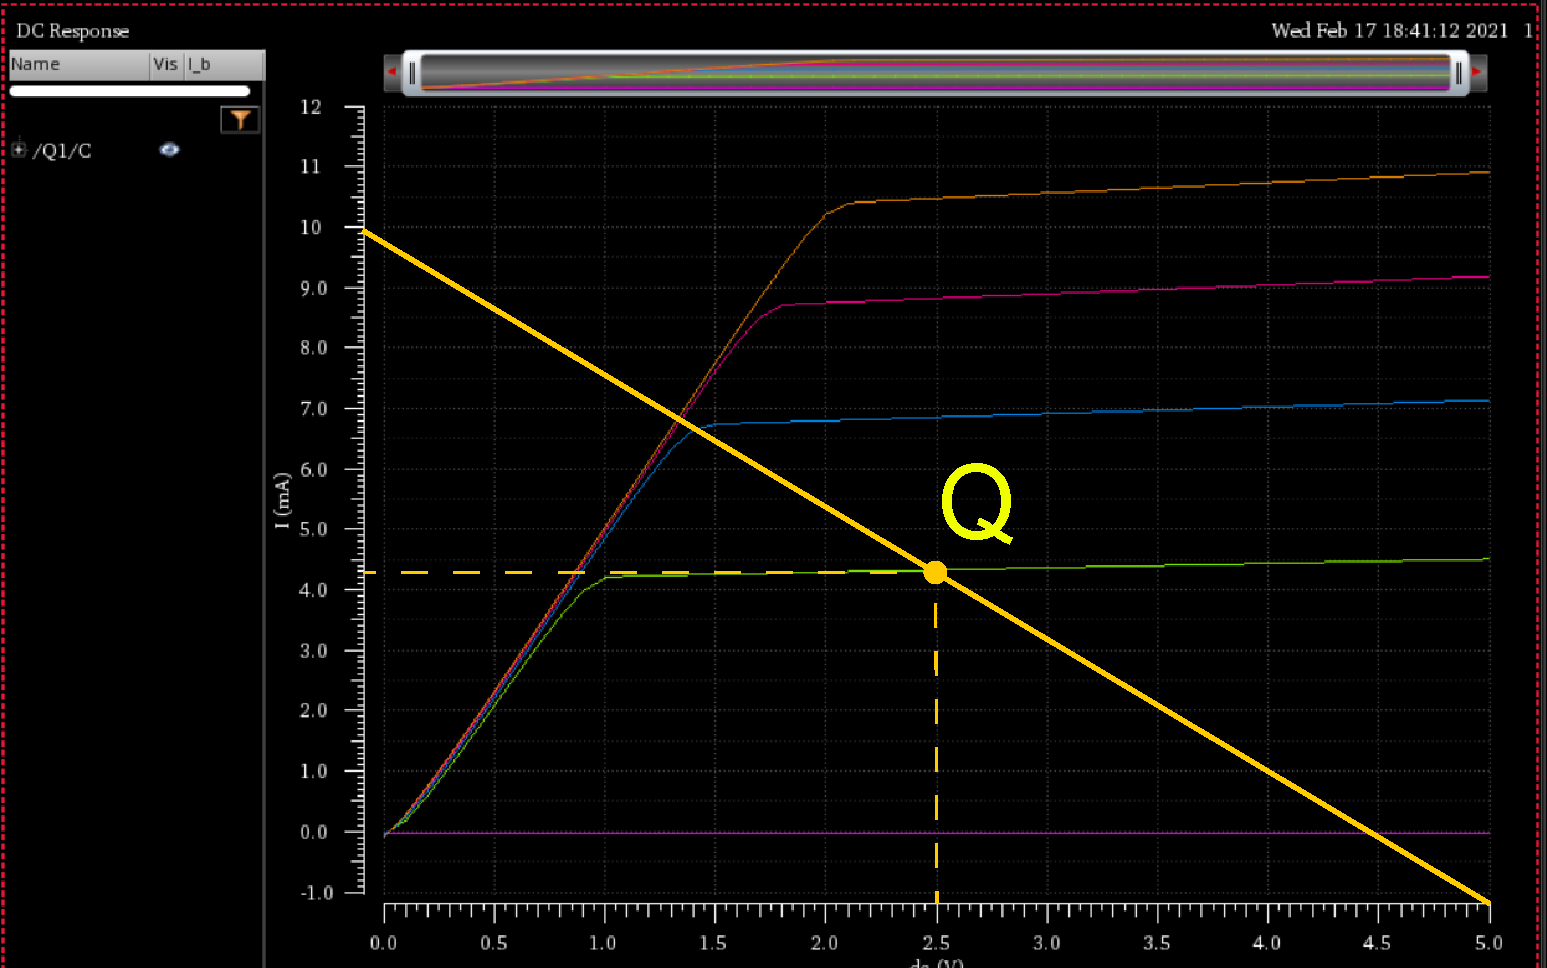
\includegraphics[width=1\linewidth]{1.png}}
\caption{Прототип схеми.}
\label{ris1}
\end{figure}
У мене за варіантом тип підкладки КЕФ, тобто n-тип підкладки, тоді і p-канал у транзисторах.\\

Тоді, можемо побудувати уже електричну схему на основі прототипу:
\begin{figure}[h!]
\center{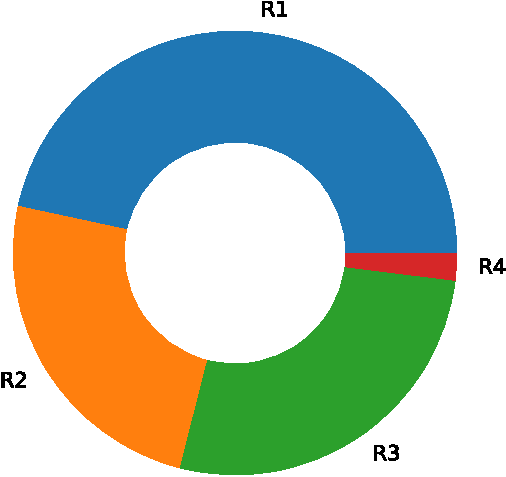
\includegraphics[width=1\linewidth]{2.png}}
\caption{Електрична схема на основі прототипу.}
\label{ris2}
\end{figure}
Так як у нас інтегральна мікросхема, то треба аби всі підклади були підключені до спільного виводу.\\
\newpage
Далі переходимо до наступного завдання. Треба скласти таблицю істинності, але легше зробити розбивши схему на каскади. Розглядати будемо спрощену модель схеми, замінивши усі транзистори змінними резисторами, окрім T4 I T5. Так як у них затвор під’єднаний до стоку, то ці транзистори будуть грати роль навантаження, тобто заміняємо їх звичайним резистором. Тоді, спрощена модель:
\begin{figure}[h!]
	\begin{center}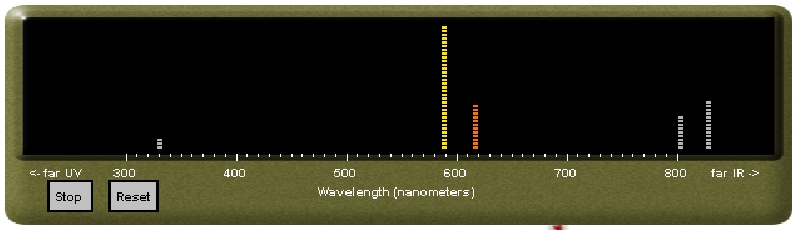
\includegraphics[width=0.7\linewidth]{3.png}\end{center}
	\caption{Спрощена модель.}
	\label{ris3}
\end{figure}


Бачимо, що у цій схемі всього три каскади. Розпочнемо з першого. У нас три змінних резистори, які можна об’єднати в один ($R_1, R_2$ і $R_3$, так як паралельно підключені). Це виглядатиме так:
\begin{figure}[h!]
	\center{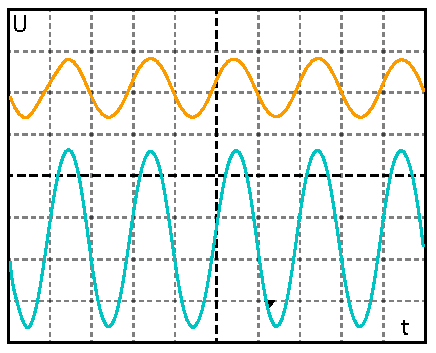
\includegraphics[width=0.6\linewidth]{4.png}}
	\label{ris4}
\end{figure}


\begin{align}
  \dfrac{1}{R_{123}} = \dfrac{1}{R_{1}}+\dfrac{1}{R_{2}} + \dfrac{1}{R_3};\\
  R_{123} = \dfrac{1}{\dfrac{1}{R_{1}}+\dfrac{1}{R_{2}} + \dfrac{1}{R_3}};
\end{align}










\clearpage
По нашому скороченню, у нас вийшов резистивний дільник напруги (по резисторам $R_{4}$ i $R_{123}$). Знаходимо напругу $U_a$.

\begin{align}
  U_a = \dfrac{R_{123}}{R_{4} + R_{123}} \cdot E
\end{align}
По цих формулах уже можемо складати таблицю істинності для першого каскаду. Так як функція не є складною, можна одразу підставляти числа і шукати опір $R_{123}$.

\begin{table}[h]
\caption{Таблиця опорів}
  \begin{center}
    \begin{tabular}{|c|c|c|c|c|c|c|c|c|}
    \hline
    $R_1 $  & 1 & 1 & 1 & 1 & 0 & 0 & 0 & 0 \\ \hline
    $R_2 $  & 1 & 1 & 0 & 0 & 1 & 1 & 0 & 0 \\ \hline
    $R_3 $  & 1 & 0 & 1 & 0 & 1 & 0 & 1 & 0 \\ \hline
$R_{123} $  & 1 & 0 & 0 & 0 & 0 & 0 & 0 & 0\\ \hline
    %$U_a  $ & 0 & 0 & 0 & 0 \\ \hline
    \end{tabular}
  \end{center}
\end{table}

1 – Це коли опір у нас наближається до нескінченності (якщо говорити за опори),а для напруг – коли вона більша за порогову напругу (коли транзистор відкритий), а 0 – це звичайний нуль, коли опір = 0, а напруга менша за порогову напругу. І підставляємо значення резисторів аби знайти Ua.\\

Тоді, загальна таблиця разом з x1, x2, x3 матиме вигляд:

\begin{table}[h]
\caption{Загальна таблиця опорів}
  \begin{center}
    \begin{tabular}{|c|c|c|c|c|c|c|c|c|}
    \hline
    $R_1 $  & 0 & 0 & 0 & 0 & 1 & 1 & 1 & 1   \\ \hline
    $R_2 $  & 0 & 0 & 1 & 1 & 0 & 0 & 1 & 1 \\ \hline
    $R_3 $  & 0 & 1 & 0 & 1 & 0 & 1 & 0 & 1 \\ \hline
    $U_a $  & 1 & 0 & 0 & 0 & 0 & 0 & 0 & 0\\ \hline
    \end{tabular}
  \end{center}
\end{table}
Усе, таблиця істинності 1 каскаду зроблена. Далі переходимо до 2 і 3 каскаду:\\
\begin{figure}[h!]
\center{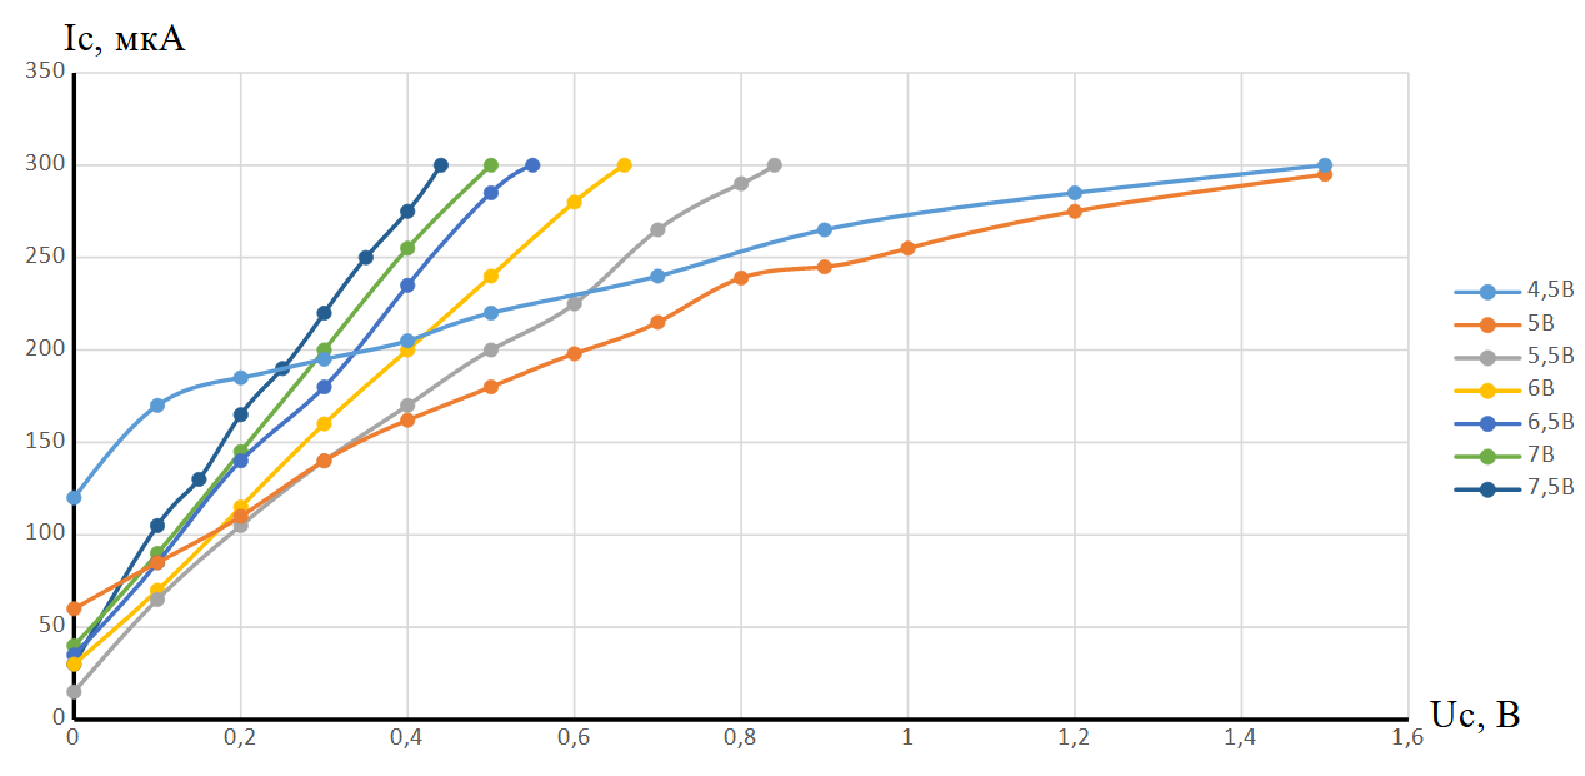
\includegraphics[width=0.5\linewidth]{5.png}}
\label{ris5}
\end{figure}

Тут два дільники напруги (2 і 3 каскад відповідно). Можемо одразу скласти формули напруги для Ub та Y:
$$ U_b = E\cdot \dfrac{R_6}{R_5+R_6}$$
$$ y = E\cdot \dfrac{R_s}{R_7+R_8}$$

Складаємо таблицю істинності одразу для двох каскадів:

\begin{table}[h]
  \begin{center}
  \begin{tabular}{|c|c|c|}
  \hline
  Ua & 1 & 0 \\ \hline
  R6 & 0 & 1 \\ \hline
  Ub & 0 & 1 \\ \hline
  R7 & 1 & 0 \\ \hline
  R8 & 0 & 1 \\ \hline
  Y  & 0 & 1 \\ \hline
  \end{tabular}
  \end{center}
\end{table}

Таблиця істинності 2 і 3 каскаду є. Тепер об’єднаємо таблиці істинності першого і другого – третього каскадів:


\begin{table}[h]
  \begin{center}
\begin{tabular}{|c|c|c|c|c|c|c|c|c|}
\hline
X1 & 0 & 0 & 0 & 0 & 1 & 1 & 1 & 1 \\ \hline
X2 & 0 & 0 & 1 & 1 & 0 & 0 & 1 & 1 \\ \hline
X3 & 0 & 1 & 0 & 1 & 0 & 1 & 0 & 1 \\ \hline
Ua & 1 & 0 & 0 & 0 & 0 & 0 & 0 & 0 \\ \hline
Ub & 0 & 1 & 1 & 1 & 1 & 1 & 1 & 1 \\ \hline
Y  & 0 & 1 & 1 & 1 & 1 & 1 & 1 & 1 \\ \hline
\end{tabular}
  \end{center}
\end{table}

Ми побачили, що другий каскад інвертуючий, через що Ub має протилежні знаки відносно Ua, а третій каскад не є інвертуючим, тому і має те саме, що Ub.
Далі складаємо логічну функцію по отриманій таблиці:
\begin{equation}
\begin{array}{c}
Y=\bar{x}_{1} \cdot \bar{x}_{2} \cdot x_{3}+\bar{x}_{1} \cdot x_{2} \cdot \bar{x}_{3}+\bar{x}_{1} \cdot x_{2} \cdot x_{3}+x_{1} \cdot \bar{x}_{2} \cdot \bar{x}_{3}+ \\
+x_{1} \cdot \bar{x}_{2} \cdot x_{3}+x_{1} \cdot x_{2} \cdot \bar{x}_{3}+\bar{x}_{1} \cdot \bar{x}_{2} \cdot \bar{x}_{3}= \\
=\bar{x}_{1} \cdot \bar{x}_{2} \cdot\left(x_{3}+\bar{x}_{3}\right)+\bar{x}_{1} \cdot x_{2} \cdot\left(\bar{x}_{3}+x_{3}\right)+x_{1} \cdot \bar{x}_{2} \cdot\left(\bar{x}_{3}+x_{3}\right)+x_{1} \cdot x_{2} \cdot \bar{x}_{3}= \\
=\bar{x}_{1} \cdot \bar{x}_{2}+\bar{x}_{1} \cdot x_{2}+x_{1} \cdot \bar{x}_{2}+x_{1} \cdot x_{2} \cdot \bar{x}_{3}=\\
\bar{x}_{1} \cdot\left(\bar{x}_{2}+x_{2}\right)+x_{1} \cdot\left(\bar{x}_{2}+x_{2} \cdot \bar{x}_{3}\right)= \\
=\bar{x}_{1}+\bar{x}_{2}+\bar{x}_{3}=\overline{x_{1} \cdot x_{2} \cdot x_{3}}
\end{array}
\end{equation}



І далі, останній крок, малюємо логічну схему по формулі:


\begin{figure}[h!]
\center{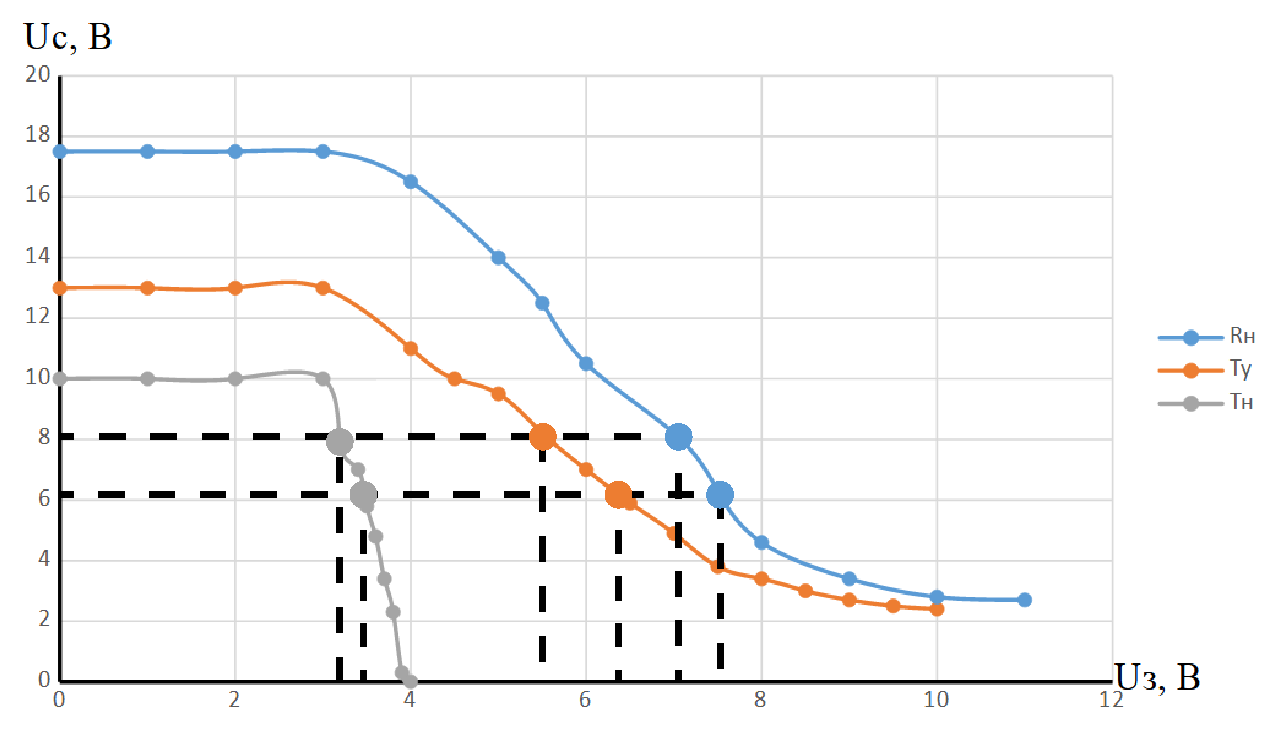
\includegraphics[width=0.9\linewidth]{6.png}}
\label{ris6}
\end{figure}


















\end{document}
